% Пример заготовки для презентации с использованием класса Beamer LaTeX.
% Версия от 09 ноября 2018 года.
\documentclass[12pt,a4paper,mathserif]{beamer}
\usepackage[utf8x]{inputenc}
\usepackage{ucs}
\usepackage[T2A]{fontenc}
\usepackage[english,russian]{babel}
\usepackage{amsmath}
\usepackage{amsfonts}
\usepackage{amssymb}
\usepackage{mathtext}
\usepackage{graphicx}
\usepackage{enumerate}
\usepackage{multirow}
\usepackage{ragged2e}
% Пакет для оформления исходного кода
\usepackage{minted}
\usepackage{adjustbox}
\justifying
\renewcommand{\raggedright}{\leftskip=0pt \rightskip=0pt plus 0cm}
\setbeamertemplate{caption}[numbered]

\usetheme {Madrid}
\usecolortheme [RGB={85, 107, 47}]{structure} %Dark Olive Green

\author[Лаптев А.В.]{{Cтудент 5.306М группы: Лаптев А.~В.}\\
{Научный руководитель: Калачев А.~В.}}
\title[Барнаул 2025]{Автоматизация решения CAPTCHA в текстовом формате}
% \subtitle{Отчет по научно-исследовательской работе}

\begin{document}
\begin{frame}
\maketitle
\end{frame}

\begin{frame}{Актуальность}
    \setlength{\parindent}{0.5cm}
    CAPTCHA давно является стандартным инструментом для защиты веб-ресурсов от спама, автоматизированных ботов и нежелательного извлечения данных.

    Автоматизированное распознавание текстовых CAPTCHA позволяет значительно снизить необходимость ручного тестирования веб-приложений, что, в свою очередь, повышает скорость и эффективность тестирования. Кроме того, подобные методы могут использоваться для анализа надёжности внедрённых CAPTCHA, выявления их слабых мест и повышения безопасности веб-приложе-\ний, например, за счёт комбинирования нескольких методов защиты.
\end{frame}

\begin{frame}{Современная реализация текстовых CAPTCHA}
    \setlength{\parindent}{0.5cm}
    Текстовые CAPTCHA обычно состоят из букв и цифр. Зачастую используются символы латинского алфавита (как прописные, так и строчные) и цифры от 0 до 9. Рекомендуемый набор символов в генераторах на некоторых CRM платформах выглядит следующим образом: ABCDEFGHJKLMNPQRSTWXYZ23456789. Длина последовательности символов обычно составляет от 4 до 8 символов.

    Для усложнения автоматического распознавания текстовые \\CAPTCHA подвергаются различным искажениям:
    \begin{enumerate}
        \item геометрические искажения;
        \item перекрытие символов;
        \item добавление шума;
        \item сложные фоны;
        \item нелинейные искажения.
    \end{enumerate}
\end{frame}

\begin{frame}{\smallАрхитектуры нейронных сетей для распознавания текста}
    \setlength{\parindent}{0.5cm}
    Для распознавания текста с переменной длиной последовательности в задачах CAPTCHA наиболее часто применяются следующие архитектуры нейронных сетей:

    \begin{enumerate}
        \item оптическое распознавание символов (OCR);
        \item рекуррентные сверточные нейронные сети (CRNN);
        \item архитектуры последовательного обучения (Seq-to-Seq).
    \end{enumerate}
\end{frame}

\begin{frame}{Выбор эффективной модели}
    \setlength{\parindent}{0.5cm}
    На начальных этапах экспериментов Seq-to-Seq-модель показала наилучшие результаты среди рассмотренных вариантов. В отличие от OCR- и CRNN-моделей, данная архитектура смогла достичь более высокой точности распознавания последовательностей символов, что обусловлено применением механизма внимания. Дальнейшая работа с моделью была сосредоточена на её оптимизации и улучшении параметров обучения.
\end{frame}

\begin{frame}{Seq-to-Seq модель. Функция потерь}
    \begin{figure}[H]
        \centering
        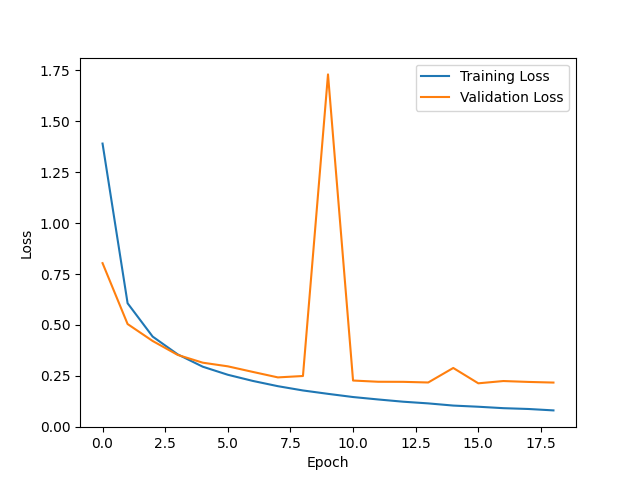
\includegraphics[width=0.7\linewidth]{imgs/Model_loss.png}
        \caption{График изменения значений функции потерь.}
        \label{fig:loss}
    \end{figure}
\end{frame}

\begin{frame}{Seq-to-Seq модель. Точность предсказаний}
    \begin{table}[H]
    \centering
    \caption{Точность предсказаний для последовательностей от 4 до 7 символов.}
    \begin{tabular}{|l|l|}
        \hline
        Длина последовательности & Точность распознавания \\
        \hline
        4 символа & 0.9305 \\
        \hline
        5 символов & 0.7450 \\
        \hline
        6 символов & 0.4575 \\
        \hline
        7 символов & 0.1915 \\
        \hline
    \end{tabular}
    \label{tab:probability}
\end{table}
\end{frame}

\begin{frame}{Seq-to-Seq модель. Матрица ошибок}
    \begin{figure}[H]
        \centering
        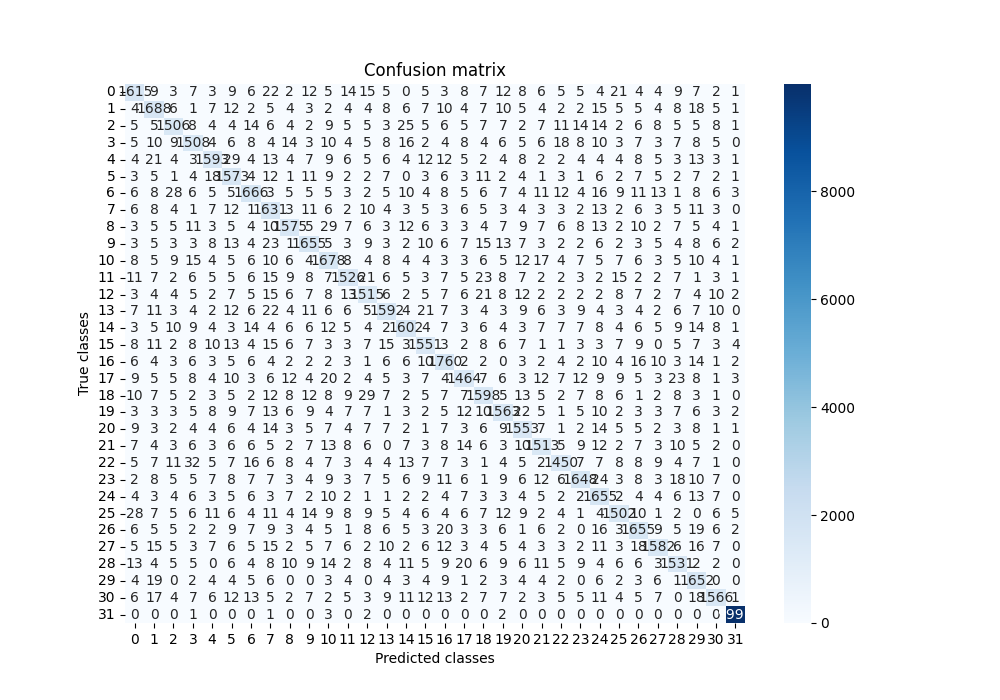
\includegraphics[width=0.85\linewidth]{imgs/Confusion_matrix.png}
        \caption{Матрица ошибок для обученной модели.}
        \label{fig:cm}
    \end{figure}
\end{frame}

\end{document}
